%% Supporting Information for "The Size of the Storm Sets the Horizon" (GRL; AGU Advances version: supplement_agu_advances.tex)
%% Compiled standalone (article class); port into the AGU SI template
%% (agutexSI2019.cls from Overleaf) at submission.
\documentclass[11pt]{article}
\usepackage[margin=1in]{geometry}
\usepackage{amsmath}
\usepackage{amssymb}
\usepackage{graphicx}
\usepackage{booktabs}
\usepackage{lineno}
\linenumbers

\title{Supporting Information for\\
``The Size of the Storm Sets the Horizon: a Scale-Aware Evaluation of AI
Precipitation Forecasts''}
\author{Sophie Abramian, Tim Zhou, Sara Shamekh}
\date{}

\begin{document}
\maketitle
\renewcommand{\thefigure}{S\arabic{figure}}

\section*{Text S1. The leakage-safe patch split}
Training samples are $128 \times 128$ non-overlapping patches tiled from
each $320 \times 1440$ frame: a $2 \times 11$ grid of 22 blocks per frame,
with the remainder (the last 64 latitude rows and 32 longitude columns)
excluded throughout. The split unit is a \emph{block-day}, the pair (day,
block location), kept together across all 96 frames of its day. The
$40 \times 22 = 880$ block-days are shuffled with a fixed seed and cut
$70/15/15$ into $616$ train, $132$ validation, and $132$ test units. Two
properties make this leakage-safe: blocks never overlap (stride equals
patch size), so no pixel appears in two splits; and all frames of one
block-day stay in one split, so the strong 15-minute temporal
autocorrelation cannot leak across splits at a fixed location. The accepted
residual risk is a storm straddling the border of two adjacent blocks
assigned to different splits; evaluation therefore restricts object
statistics to systems whose centroid falls in a held-out test block. Both
model families --- deterministic and flow --- are trained on the identical
split. An earlier day-level split leaked through temporal autocorrelation
and was discarded; no result in the paper uses it.

\section*{Text S2. Architecture and training details}
The shared trunk is a five-stage encoder--decoder: each stage two
$3{\times}3$ convolutions with GroupNorm (8 groups) and ReLU and 0.05
Dropout2d, channels $64 \rightarrow 1024$ with $2\times$ max pooling, a
$2048$-channel bottleneck at $4^2$, transpose-convolution upsampling with
skip concatenations ($124.6$~M parameters for the two-head model). The
two-head loss is $\mathrm{total} = \mathrm{MSE}_{\mathrm{wet}} +
1.0\,\mathrm{BCE} + 0.25\,\mathrm{FSS}$: a masked intensity MSE on wet
pixels (in mm), binary cross-entropy on the wet/dry logits over the full
field, and a differentiable fractions-skill-score term at kernel sizes
$[1, 3, 5, 11, 19, 33]$ pixels --- chosen to coincide with the paper's
$L$ bins at $27.8$~km per pixel --- with wet threshold $0.1$~mm and sigmoid
sharpness 20. Training: AdamW ($10^{-3}$, weight decay $10^{-5}$), StepLR
(halving every 8 epochs), batches of 64 patches, early stopping after 10
epochs without validation improvement (51--82 epochs per lead), a single
A100 per run, fixed seed. One model per lead
($0.25, 0.5, 1, 2, 3, 6$~h). The flow's velocity network reuses the trunk
with an eleventh input channel (the flow state $x_s$), FiLM conditioning on
the flow time $s$, and a
single unactivated velocity head; the per-lead noise scale $\sigma$ is the
measured wet-masked forecast error rms in log-rain space
($0.102, 0.119, 0.146, 0.171, 0.188, 0.204$ for the six leads).

\textbf{Inputs.} Each input field is standardized with one mean and one
standard deviation per field over the whole record; the rain is
transformed to $\ln(1 + R)$ before standardization, $R$ in mm per
$15$~min. The target is the rain in mm, not standardized. The models see
one $128 \times 128$ block at a time and nothing outside it. In addition to
the ten fields, the U-Net receives at its bottleneck the mean and the
minimum of the outgoing longwave radiation over the block: two numbers that
tell it how much deep convection the block holds and how cold its highest
tops are.

\textbf{U-Net loss.} The loss is Eq.~1 of the main text, with weights
$1$, $1$, and $0.25$; the wet threshold of the fraction term is
$0.1$~mm, with a sigmoid of sharpness $20$ to keep it differentiable, and
its six windows ($1, 3, 5, 11, 19, 33$ pixels) coincide with the size
bands of the evaluation. The wet/dry head hedges like the rain head:
because some rain is present almost everywhere in a $15$-min
kilometer-scale field, it calls almost every pixel wet (Figure~S1). The
evaluation uses the rain head alone.

\textbf{Flow matching.} The flow works in the log space $z = \ln(1 + R)/2$.
For one training sample with inputs $c$, U-Net forecast $z_{\mathrm{fc}}$,
and truth $z$, the start is $x_0 = z_{\mathrm{fc}} + \sigma\varepsilon$
with $\varepsilon \sim \mathcal{N}(0, I)$, the end is $x_1 = z$, and
$x_s = (1 - s)\,x_0 + s\,x_1$. The velocity network is the least-squares
fit of
\begin{equation}
v_s(x, c) = \mathbb{E}\big[\,x_1 - x_0 \;\big|\; x_s = x,\, c\,\big] :
\end{equation}
the average, over all training lines passing through $x$ at time $s$, of
the direction to their own truth. A draw starts from
$y_0 = z_{\mathrm{fc}} + \sigma\varepsilon$ and integrates
$y_1 = y_0 + \int_0^1 v_s(y_s, c)\,\mathrm{d}s$ with $32$ Heun steps (the
last a plain Euler step). Besides generating different draws, the noise
spreads the starting points of the training lines around each forecast,
so that a new forecast starts where training lines have passed. All flow
statistics are computed on one draw per block and frame with a fixed seed,
never on an average of draws.

\section*{Text S3. The warm-started diffusion model as a sampling sensitivity}
Before the rectified flow, the generative representative was a conditional
denoising diffusion model trained to denoise noised \emph{truth}, sampled by
warm-starting from the noised deterministic \emph{forecast} (SDEdit-style)
with a lead-dependent noise budget calibrated per lead. This retrofit
carries a train/test mismatch --- the network never saw noised forecasts
during training --- and it shows: across noise budgets the small-scale
spectral power saturates at $0.80$--$0.85$ of the truth's and the wet area
falls ${\sim}20\%$ short at $6$~h. The flow, trained natively on the
forecast$\to$truth transport, clears this ceiling (band ratio $1.115$, wet
area $+1.5\%$ at $6$~h). We therefore report the diffusion model as a
sampling-protocol sensitivity: its failure localizes the DDPM's limit in
the sampler's mismatch, not in an informational limit of the inputs.

\section*{Text S4. The detection horizon}
Systems are counted in ten log-spaced size bands from $25$ to $600$~km
(Figure~4a,b of the main text) or $800$~km (Figure~4c,d). In each band, the
POD at the six leads is divided by its value at the shortest lead,
$15$~min, and $\exp[-(t - 0.25\,\mathrm{h})/\tau]$ is fitted to the ratio
by least squares, with $\tau$ bounded to $[0.1, 200]$~h. The power law
$T(L) \propto L^{\alpha}$ is fitted by unweighted least squares of
$\ln\tau$ on $\ln L$ over the six bands from $59$ to $336$~km, the same
for the three forecasts. The two smallest bands are left out because their
systems are one to two pixels wide; the two largest because their $\tau$
exceeds the $6$~h covered by the leads several times over ($26$~h and
more), so that their values are extrapolations. Matched-pair errors
(Eq.~4 of the main text) are averaged with weights given by the truth
system's rain, in three bands: below $65$~km, $65$ to $200$~km, and above
$200$~km.

\section*{Text S5. Sensitivities of the matching}
\textbf{IoU threshold.} Storms are long-lived, so at $\mathrm{IoU} \ge 0.1$
an old storm often still overlaps its past self; loose matching therefore
flatters persistence at short leads. Tightening the acceptance threshold
lowers persistence detection faster than either model's and does not change
the ordering of the three forecasts or the sign of the flow's margin.
\textbf{Rain threshold.} At the km scale the object population is stable
around the $0.1$~mm threshold. On the $0.25^{\circ}$ WB2 grid the
rate-equivalent threshold ($2.4$~mm per $6$~h $= 0.1$~mm per $15$~min)
is required: at $0.1$~mm per $6$~h the drizzle field percolates into a
single belt-spanning system. The POD-by-scale shape is robust across
thresholds $0.1$--$2.4$~mm per $6$~h (FAR $0.71 \rightarrow 0.39$).
\textbf{One-to-one matching.} Greedy one-to-one assignment penalizes a
model that splits one true system into several (each fragment beyond the
first counts as a false alarm and the area error reads low). This affects
the sharp GenCast member on the coarse grid, which over-segments (804
forecast objects against 444 in ERA5 truth on a reference day, with wet
coverage correct at $8.6\%$ for all models), so the member's negative
$\mathrm{d}\ln A$ is in part a matching artifact; the smooth deterministic
models under-segment instead ($\approx 200$ objects). A many-to-one variant
is the appropriate sensitivity and does not change the intensity-bias
conclusions.

\clearpage
\begin{figure}
\centering
A.\\
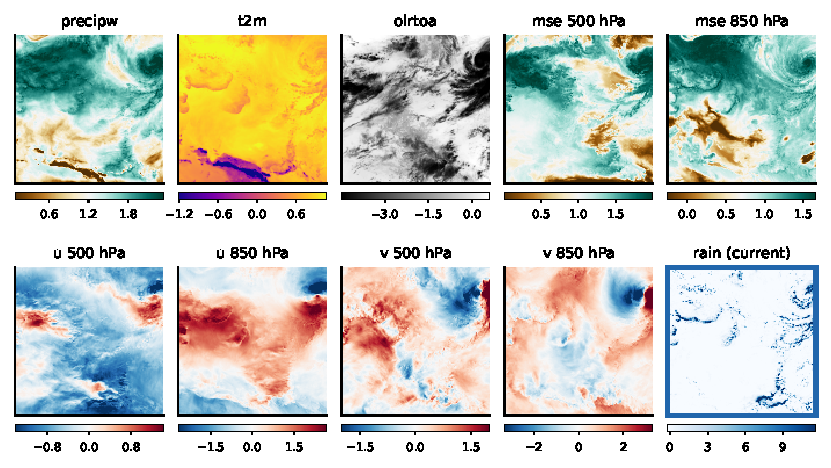
\includegraphics[width=\textwidth]{figures/fig2a_inputs.pdf}\\[2mm]
B.\\
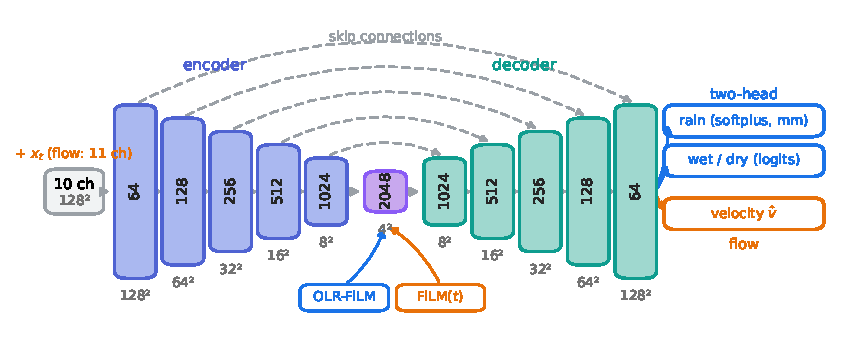
\includegraphics[width=\textwidth]{figures/fig1b_architecture.pdf}\\[2mm]
C.\\
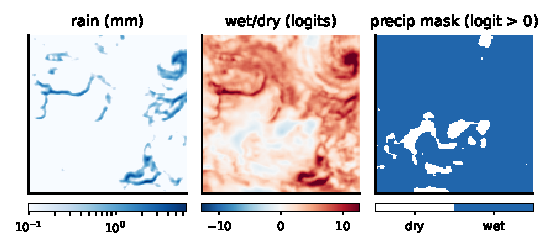
\includegraphics[width=0.42\textwidth]{figures/fig2c_outputs.pdf}
\caption{\textbf{The two-head U-Net, input to output} (the standard example
block). A.~The ten input channels, concatenated in this order with the
current rain last (blue frame --- the persistence forecast handed to the
model, which nests the null); each map standardized, colormaps by family
(moisture and moist static energy brown--teal, temperature thermal, OLR
grayscale with cold convective tops dark, winds red--blue, rain blue on a
log scale). B.~The trunk: five encoder stages (each two $3{\times}3$
convolutions, GroupNorm, ReLU) from $64$ channels at $128^2$ down to $1024$
at $8^2$, a $2048$-channel bottleneck at $4^2$, a mirrored decoder with skip
concatenations, and two parallel $1{\times}1$ output heads.
C.~The outputs for this input at $+3$~h: the rain field (softplus, mm), the
wet/dry logits (red positive, wet-leaning; blue negative, dry), and the
precipitation mask at the paper's wet threshold (rain $> 0.1$~mm) --- the
mask the object detection of Section~2.3 of the main text operates on. The
logit head itself is permissive --- trained against $y > 0$, any rain at
all, it flags wet nearly everywhere and only confidently dry regions go
negative --- so segmentation uses the rain field. The bottleneck is
conditioned by \emph{OLR-FiLM} (FiLM: Feature-wise Linear Modulation): the
patch's mean and minimum outgoing longwave radiation pass through a small
MLP that returns per-channel scale and shift $(\gamma, \beta)$ applied to
the bottleneck features --- a convective-regime gate (cold, deep tops vs
warm, shallow ones).}
\label{fig:s1}
\end{figure}

\begin{figure}
\centering
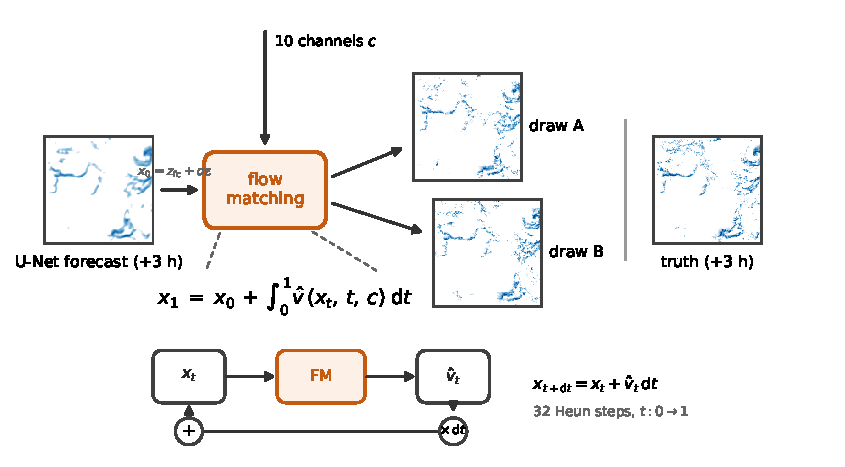
\includegraphics[width=\textwidth]{figures/fig3_flowsketch.pdf}
\caption{\textbf{Flow matching, forecast to draws} ($+3$~h, the standard
example block; all rain maps share one log color scale). The smooth two-head
forecast, perturbed by its own measured error
($x_0 = z_{\mathrm{fc}} + \sigma\varepsilon$), enters the flow-matching
module conditioned on the ten input channels $c$; each noise draw
$\varepsilon$ yields a different sharp realization (draw A, draw B) of the
same truth --- the draws differ from each other exactly where the outcome is
uncertain. Below, the module unpacked: the transport equation
$x_1 = x_0 + \int_0^1 \hat{v}(x_t, t, c)\,\mathrm{d}t$, integrated by the
unrolled loop at the bottom --- the velocity network FM reads the current
state $x_t$ (and $t$, $c$), returns $\hat{v}_t$, and the state advances by
$\hat{v}_t\,\mathrm{d}t$, repeated for $32$ Heun steps from $t = 0$ to
$1$.}
\label{fig:s2}
\end{figure}

\begin{figure}
\centering
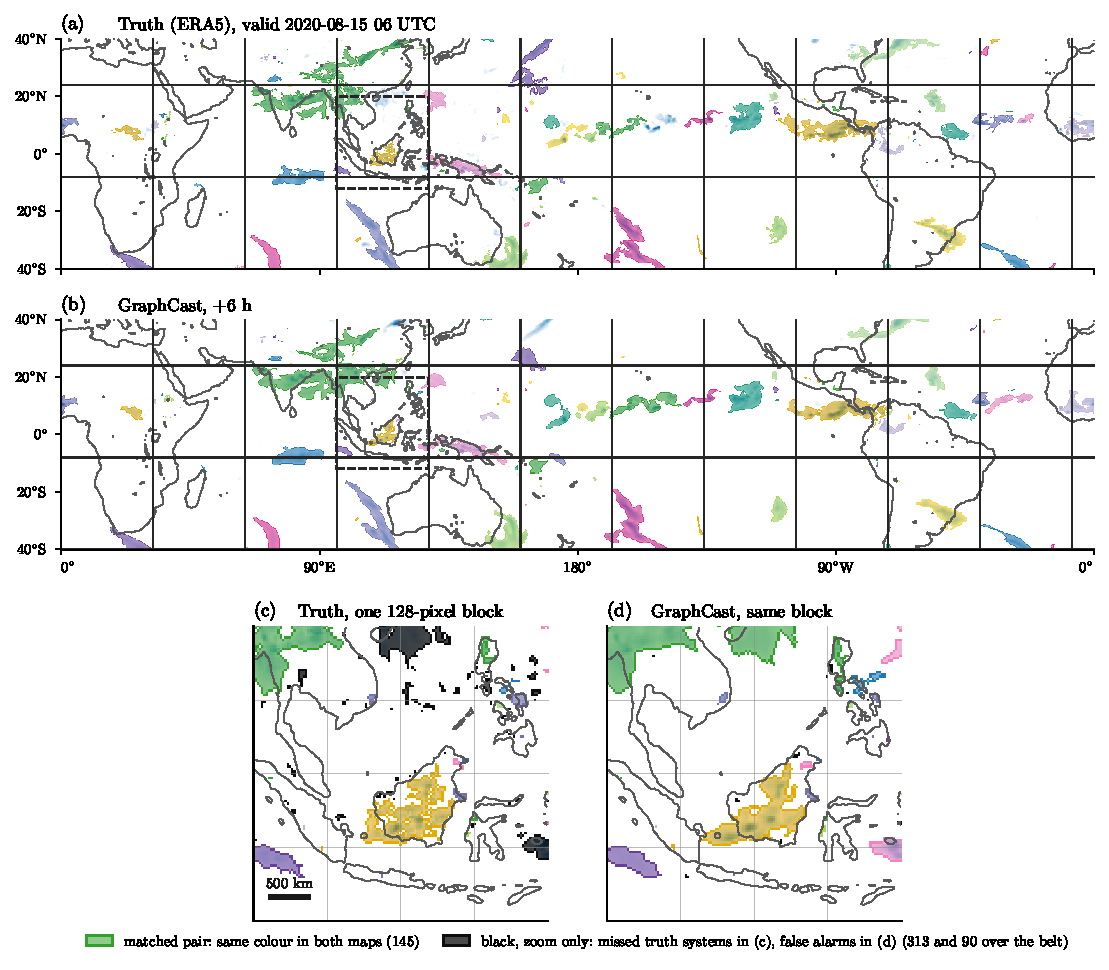
\includegraphics[width=\textwidth]{figures/figS_wb2_belts.pdf}
\caption{Object matching for GraphCast at a $6$~h lead against ERA5 over
the whole tropical belt, valid 2020-08-15 06 UTC, with the threshold and
matching of Figure~5 of the main text. (a, b) The belt on the block grid
of Figure~1; matched pairs share a color across the two maps ($145$
pairs); the dashed box marks the block of Figure~5a,b. (c, d) That block,
with the missed truth systems in (c) and the false alarms in (d) in black
($313$ and $90$ over the belt).}
\label{fig:s3}
\end{figure}

\begin{figure}
\centering
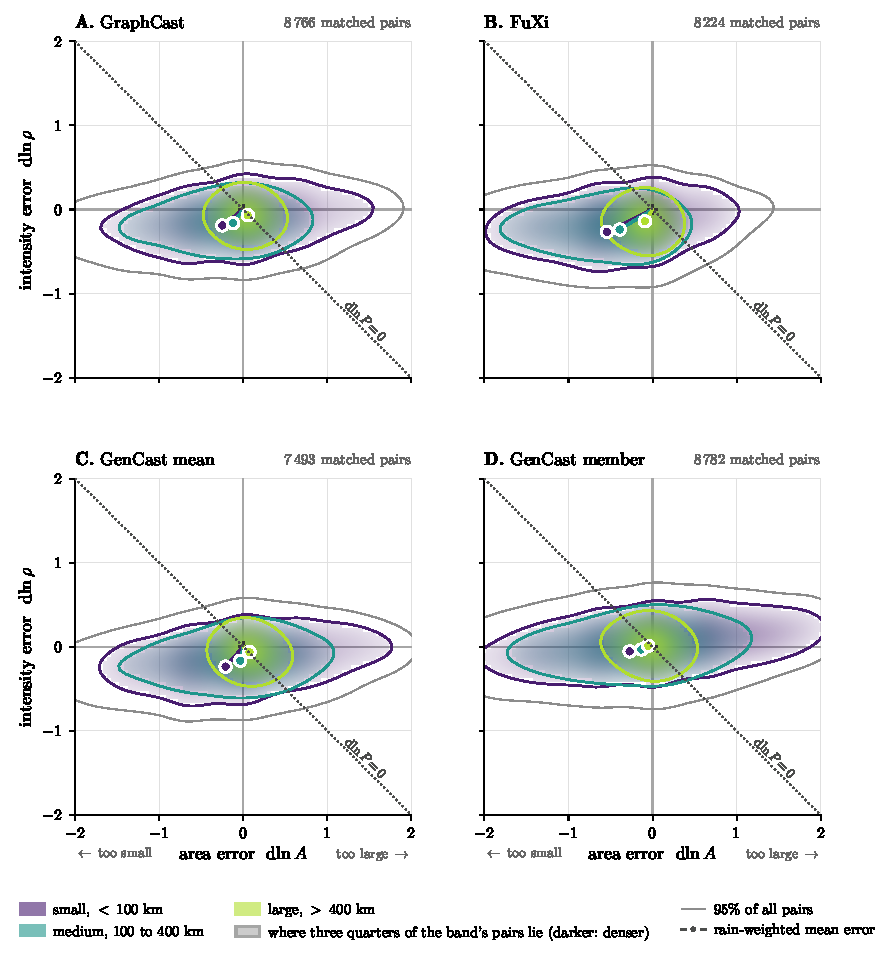
\includegraphics[width=\textwidth]{figures/fig7c_clouds.pdf}
\caption{Area and intensity errors of the matched systems for the
WeatherBench~2 models at a $12$~h lead, pooled over August 2020 (about
$8{,}000$ pairs per model), with the conventions of Figure~3 of the main
text and size bands of $<100$, $100$--$400$, and $>400$~km. The error
clouds are wide in area and narrow in intensity, the reverse of the
kilometer-scale clouds: at $0.25^{\circ}$ the rain rate is recovered and
the boundaries of the systems are not. The rain-weighted mean intensity
error of the deterministic models is $-0.24$, $-0.17$, and $-0.06$ from
the smallest to the largest band, against $-0.06$, $-0.03$, and $+0.01$
for the GenCast member.}
\label{fig:s4}
\end{figure}

\begin{figure}
\centering
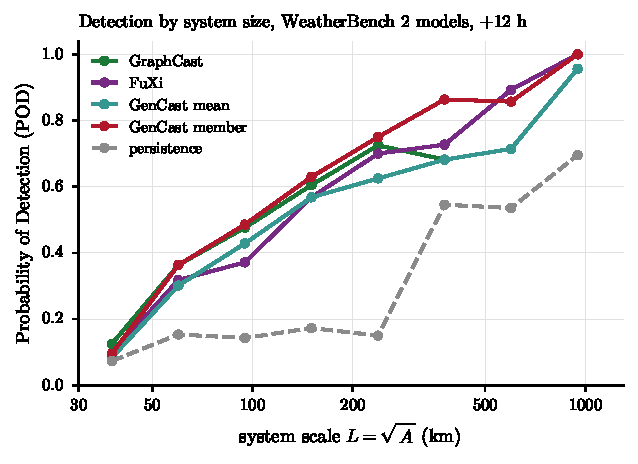
\includegraphics[width=\textwidth]{figures/fig7b_pod.pdf}
\caption{(a) Probability of detection and (b) false-alarm ratio against
system size for the WeatherBench~2 models and persistence at a $12$~h lead
(2020-08-15, two initializations), with the threshold and matching of
Figure~5 of the main text; bands with fewer than $20$ systems are blank.
Above $240$~km, one GenCast member detects $0.78$ to $0.82$ of the systems,
against $0.68$ to $0.73$ for GraphCast, with a false-alarm ratio of $0.32$
against $0.17$.}
\label{fig:s5}
\end{figure}
\end{document}
